\section{Scattering}
\label{sec:scattering}

The use of scattering techniques to probe soft condensed matter systems is commonplace.
In this work, we have focussed on the use of small angle scattering (SAS), reflectometry, and grazing incidence small angle scattering (GiSAS) techniques.
These are particularly appropriate for application to soft condensed matter systems due to the length scales capable of being probed being similar to the persistence length of the soft condensed matter systems.
The length scale covered for such techniques is from around \SI{1}{\nano\metre} to \SI{300}{\nano\metre}, as is shown in Figure~\ref{fig:lengths}.
The focus is on the equilibrium structure(s) of a material, and therefore there is no interest in the system dynamics, meaning that exclusively elastic scattering techniques may be used, where there is no energy transfer between the probing radiation and the material.
This is in contrast to inelastic scattering where energy transfer occurs; facilitating the measurement of system dynamics, such as the dynamical modes of polymers and lipid bilayers \cite{garcia_sakai_quasielastic_2009, farago_recent_2009}.
%
\begin{figure}
    \centering
    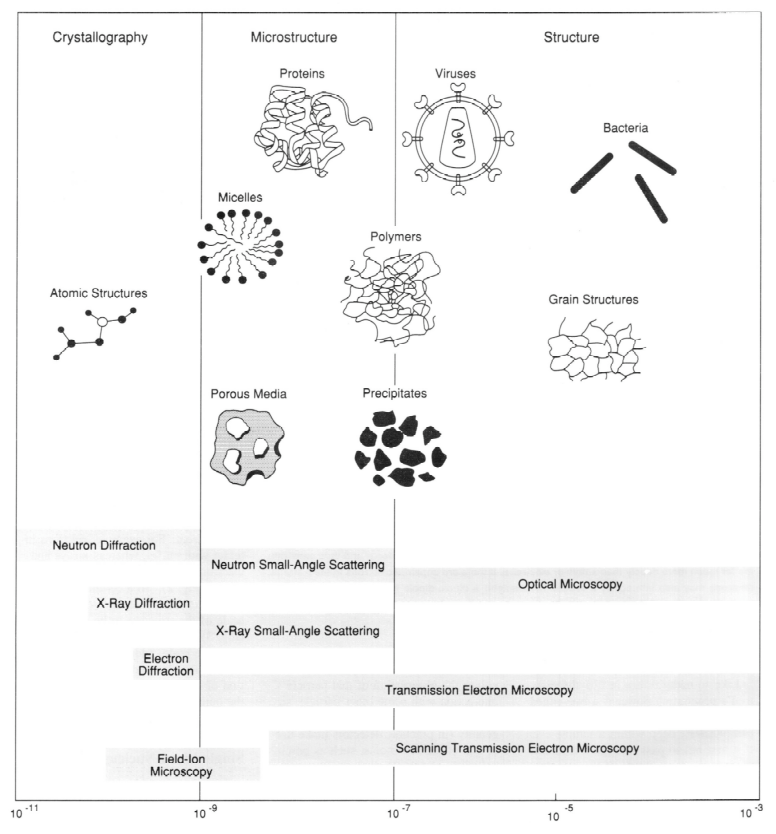
\includegraphics[width=0.85\textwidth]{theory/length}
    \caption{A representation of how different techniques can be used to probe various length scales. Reproduced, with permission of Oxford University Press\textsuperscript{\textcopyright}, from Reference~\cite{sivia_elementary_2011}.}
    \label{fig:lengths}
\end{figure}
%

Both X-ray and neutron scattering techniques are discussed and used in this work.
From an experimental viewpoint, there are significant differences between an X-ray scattering and a neutron scattering experiment.
However, there is little variation in terms of the data analysis, where the differences are limited to; the nature of the scattering lengths (see Section~\ref{convar}), and the higher background that is present in the neutron scattering experiments.

\subsection{The scattering vector}

The scattering of some probing radiation, by some sample, can be represented as shown in Figure~\ref{fig:scat}.
Since only elastic scattering is being considered, there will be no change in the frequency of the radiation, $\omega_i = \omega_f$.
This means that only the wavevector, $\mathbf{k}$, can change, $\mathbf{k}_i\neq \mathbf{k}_f$.
The difference between the incident and final wavevectors is the scattering vector, $\mathbf{q}$, where,
%
\begin{equation}
    \mathbf{q} = \mathbf{k}_i - \mathbf{k}_f.
\end{equation}
%
%
\begin{figure}
    \centering
    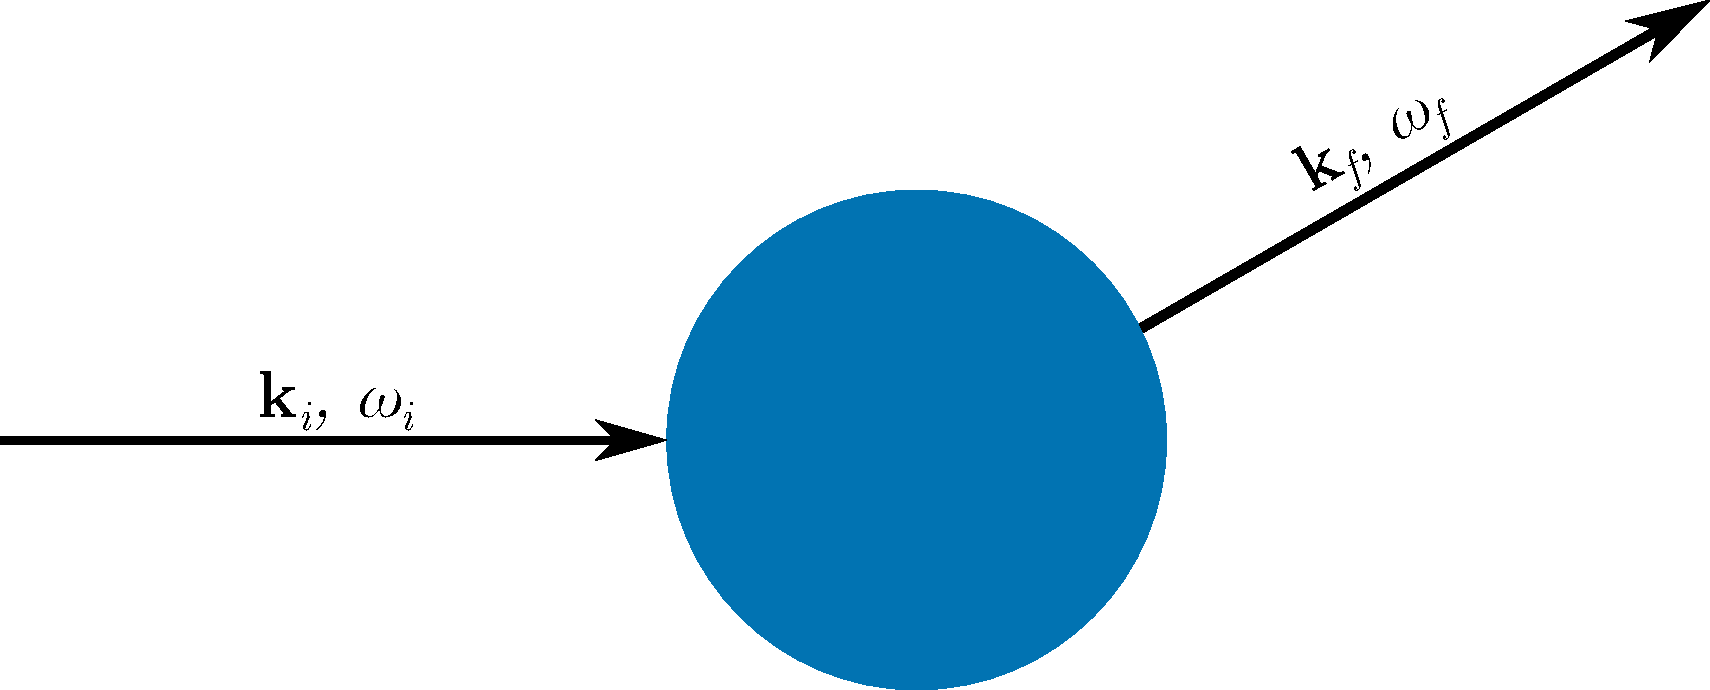
\includegraphics[width=0.85\textwidth]{theory/scat}
    \caption{A schematic of the scattering of some probing radiation by a sample (blue circle). Adapted, with permission of Oxford University Press\textsuperscript{\textcopyright}, from Reference~\cite{sivia_elementary_2011}.}
    \label{fig:scat}
\end{figure}
%
The scattering vector strictly has units of \si{\per\meter}, however it is often more practical to use \si{\per\nano\meter} or \si{\per\angstrom}.
Throughout this work, units of reciprocal \AA ngstrom will be wherever possible.
Since the frequency of the probing radiation does not change during an elastic scattering event, the wavelength, $\lambda$, will also not change, meaning that the moduli of the incident and final wavevectors are,
%
\begin{equation}
    |\mathbf{k}_i| = |\mathbf{k}_f|=\frac{2\pi}{\lambda}.
    \label{equ:wavevec}
\end{equation}
%
This means that only the angle will change during the elastic scattering event.
The vector diagram in Figure~\ref{fig:scatvec} can be used to describe the geometry of an elastic scattering event.
From this, and Equation~\ref{equ:wavevec}, the value of $q$, where $q = |\mathbf{q}|$ can be shown as,
%
\begin{equation}
    q = \frac{4\pi\sin{\theta}}{\lambda}.
    \label{equ:theq}
\end{equation}
%
%
\begin{figure}
    \centering
    
\includegraphics[width=0.85\textwidth]{theory/scatvec}
    \caption{A vector diagram describing an elastic scattering event, where $\mathbf{k}_i$ is the incident wavevector, $\mathbf{k}_f$ is the final wavevector, $2\theta$ is the scattering angle, and $\mathbf{q}$ is the scattering vector. Adapted, with permission of Oxford University Press\textsuperscript{\textcopyright}, from Reference~\cite{sivia_elementary_2011}.}
    \label{fig:scatvec}
\end{figure}
%
However, this fails to fully capture the three dimensional nature of the scattering event.
Hence, it is necessary to describe the scattering with spherical coordinates, $2\theta$, and $\phi$, such that the incoming and outgoing radiation can be described as,
%
\begin{equation}
    \begin{aligned}
        \mathbf{k}_i & = \bigg(0, 0, \frac{2\pi}{\lambda}\bigg), \\
        \mathbf{k}_f & = \frac{2\pi}{\lambda}(\sin{2\theta}\cos{\phi}, \sin{2\theta}\sin{\phi}, \cos{2\theta}),
    \end{aligned}
\end{equation}
%
where, $|\mathbf{k}_f| = \sfrac{2\pi}{\lambda}$. This allows the scattering vector to be written,
%
\begin{equation}
    \mathbf{q} = \frac{4\pi\sin{\theta}}{\lambda}(-\cos{\theta}\cos{\phi}, -\cos{\theta}\sin{\phi},\sin{\theta}).
\end{equation}
%
For an isotropic scattering pattern, it is the magnitude of the scattering vector, $q$, that is measured.
In practical terms, the scattering vector allows for easy comparison of measurements made at different radiation wavelengths.

The basic quantity measured in a scattering experiment is the differential cross section, $\sfrac{\text{d}\sigma(q)}{\text{d}\Omega}$.
This is the fraction of particles of probing radiation that is scattered with a particular set of polar coordinates, $2\theta$ and $\phi$,
%
\begin{equation}
    \frac{\text{d}\sigma(q)}{\text{d}\Omega} = \frac{R(2\theta,\phi)}{NV\Phi\Delta \Omega},
    \label{equ:dsc}
\end{equation}
%
where, $R(2\theta,\phi)$ is the rate of arrival of the scattered particles at the position $2\theta$, $\phi$, $V$ is the illuminated volume of the sample, $\Phi$ is incident flux, $\Delta \Omega$ is some small solid angle, and $N$ is the number of scattering particles of interest, in the case of elastically scattered radiation, $N = N\%_{\text{el}}$, where $\%_{\text{el}}$ is the fraction of elastically scattered radiation.

\subsection{Scattering from a single fixed particle}

It is possible to describe a steady stream X-ray photons or neutrons of wavelength, $\lambda$, travelling through space as follows,
%
\begin{equation}
    \psi_i = \psi_o \exp{(\mathbf{i} kz)},
    \label{equ:wave}
\end{equation}
%
where, $z$ is the direction of travel, and the incident flux is the magnitude of the wave squared, $\Phi = |\psi_o|^2$.
This wave then interacts with a single fixed particle elastically, propagating the wave radially outwards (Figure~\ref{fig:singleatom}).
This propagation is centred on the atom, therefore the wavevector, $\mathbf{k_f}$ is parallel to the displacement vector, $\mathbf{r}$, and the following holds,
%
\begin{equation}
    \exp{(\mathbf{i}\mathbf{k}_f\cdot \mathbf{r})} = \exp{(\mathbf{i}kr)}.
\end{equation}
%
This final wave is no longer collimated and therefore diminishes with distance, $r$.
Hence the final scattered wave has the form,
%
\begin{equation}
    \psi_f = \psi_o b\frac{\exp{(\mathbf{i}kr)}}{r},
\end{equation}
%
where, $b$ is the scattering length discussed in Section~\ref{convar}.
%
\begin{figure}
    \centering
    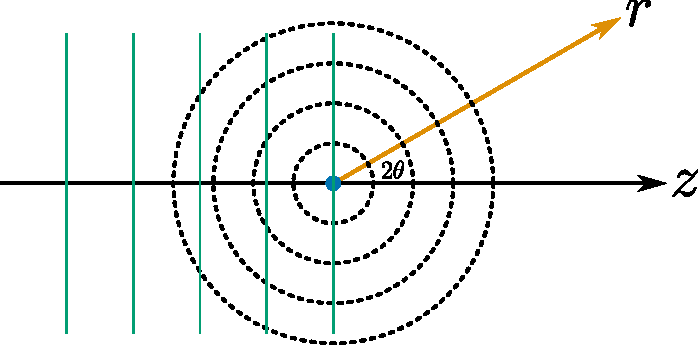
\includegraphics[width=0.85\textwidth]{theory/singleatom}
    \caption{A schematic showing the propagation of the wave of probing radiation (green lines) radially outwards following the scattering event, where $r$ is the magnitude of the displacement vector. Adapted, with permission of Oxford University Press\textsuperscript{\textcopyright}, from Reference~\cite{sivia_elementary_2011}.}
    \label{fig:singleatom}
\end{figure}
%

\subsection{Scattering from multiple particles}
\label{sec:multiscat}

It is important to consider how the probing radiation would interact with a real system, consisting of many particles.
If the incident beam has the form of Equation~\ref{equ:wave}, with the wavevector $\mathbf{k}_i = (0, 0, k)$, each particle, $j$, will contribute the following to the total scattered wave, $psi_f$, made up of the scattering from all, $N$, atoms,
%
\begin{equation}
    [\delta\psi_f]_j = \psi_o\exp{(\mathbf{ik}_i\cdot \mathbf{R}_j)}b_j\frac{\exp{\big\{\mathbf{ik}_f\cdot (\mathbf{r}-\mathbf{R}_j)\big\}}}{|\mathbf{r}-\mathbf{R}_j|},
\end{equation}
%
where, $\mathbf{R}_j$ is the position of particle $j$, $\mathbf{r}$ is some arbitrary position, and $\mathbf{k}_f$ is the wavevector of the scattered wave (Figure~\ref{fig:multiatom}).
This allows the total scattered wave to be defined as a summation of the contributions from the individual waves,
%
\begin{equation}
    \psi_f = \psi_o \exp{(\mathbf{ik}_f\cdot\mathbf{r})}\sum_{j=1}^{N}\bigg\{b_j \frac{\exp{(\mathbf{iq}\cdot \mathbf{R}_j)}}{|\mathbf{r}-\mathbf{R}_j|}\bigg\}.
    \label{equ:scatter}
\end{equation}
%
Equation~\ref{equ:scatter} holds true, within the Born approximation, where the scattered wave has no impact on the incident wave and each wave is scattered only once.
%
\begin{figure}
    \centering
    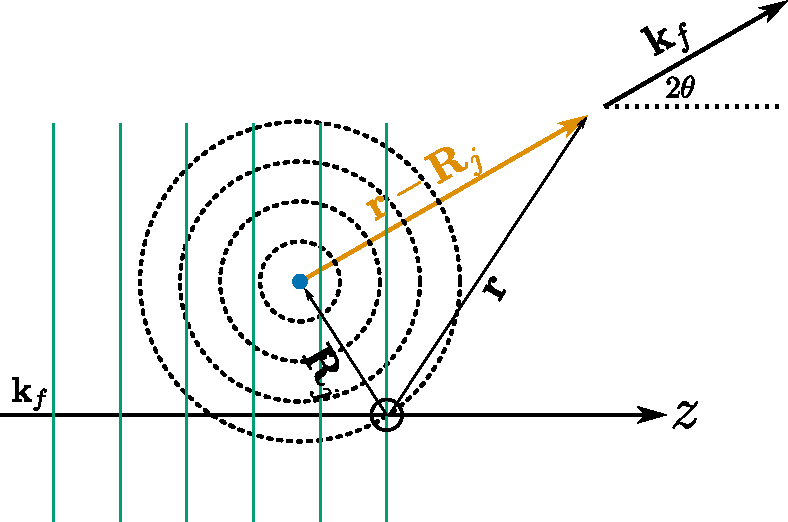
\includegraphics[width=0.85\textwidth]{theory/multiatom}
    \caption{A schematic showing the interaction of radition scattered by two particles that are separated by the vector $\mathbf{R}_j$. Adapted, with permission of Oxford University Press\textsuperscript{\textcopyright}, from Reference~\cite{sivia_elementary_2011}.}
    \label{fig:multiatom}
\end{figure}
%

The sample-detector distance is usually much larger than the typical particle size, allowing for the following approximation,
%
\begin{equation}
    |\mathbf{r} - \mathbf{R}_j| = |\mathbf{r}| = r.
\end{equation}
%
This is termed the Fraunhofer, or far-field limit, and allows Equation~\ref{equ:scatter} to be simplified,
%
\begin{equation}
    |\psi_f|^2 = \frac{\Phi}{r^2}\Bigg|\sum_{j=1}^{N}b_j\exp{(\mathbf{iq}\cdot\mathbf{R}_j)}\Bigg|^2.
\end{equation}
%
In the scattering experiment, radiation is deflected elastically into a detector with a small area, $\delta A$, with the polar coordinates, $2\theta$ and $\phi$, at a rate of $R_{\text{el}}$,
%
\begin{equation}
    R_{\text{el}}(2\theta,\phi) = |\psi_f|^2\delta A = \Phi\delta\Omega\Bigg|\sum_{j=1}^{N}b_j\exp{(\mathbf{iq}\cdot\mathbf{R}_j)}\Bigg|^2,
\end{equation}
%
where, $\delta\Omega = \sfrac{\delta A}{r^2}$.
Therefore, the differential cross section, defined in Equation~\ref{equ:dsc} can be related to the scattering from the sample as,
%
\begin{equation}
    \bigg(\frac{\text{d}\sigma(q)}{\text{d}\Omega}\bigg)_{\text{el}} = \frac{1}{V} \Bigg|\sum_{j=1}^{N}b_j\exp{(\mathbf{iq}\cdot\mathbf{R}_j)}\Bigg|^2.
    \label{equ:sca}
\end{equation}
%

\subsection{Scattering length density}
\label{sec:sld}

While it may be helpful to consider the scattering from multiple particles individually, where each particle has a scattering length, $b$.
In practice, due to the low experimental resolution at small angles, it is more common to consider the scattering length density, $\rho$, of the system,
%
\begin{equation}
    \rho = \frac{1}{V}\sum_{i=0}^{N} b_i,
\end{equation}
%
where $N$ is the total number of particles in the volume $V$.
A result of this equation is the ability to rewrite Equation~\ref{equ:sca} as,
%
\begin{equation}
    \bigg(\frac{\text{d}\sigma(q)}{\text{d}\Omega}\bigg)_{\text{el}} = \frac{1}{V} \Bigg|\iiint \limits_V \rho\exp{(\mathbf{iq}\cdot\mathbf{R})}\text{d}^3\mathbf{R}\Bigg|^2.
    \label{equ:sldsca}
\end{equation}
%
This above equation shows that the scattering differential cross-section from some object is related to the scattering length density profile of that object by a Fourier transform.

\subsection{Model-dependent analysis}

All types of scattering patterns can be analysed by one of two methods; model independent and model-dependent.
The nature of this work means that it will focus on model-dependent analysis methods, often where the model is derived from some atomistic, or coarse-grained simulation. Model-dependent analysis has significant benefits over model-independent methods, such as improved resolution and more detailed information about the structure.
However, the necessity of the inclusion of \emph{a priori} information within model-dependent analysis may act to bias the result.
While this is undesirable, these assumptions can, and should, be educated based on the chemical information present, such as the propensity for twin-tailed lipid molecules to form monolayers at an air-water interface \cite{mccluskey_model-dependent_2018}.

The scattering from the model system is determined, using technique specific methods that are discussed in detail in later sections.
This is then compared with the experimental data using some goodness-of-fit metric, the model is then varied to find the best possible model for the data provided using some optimisation algorithm.
In order to accurately reproduce the experimental measurement, it is necessary to include some instrumental resolution function, $res(q)$, in the modelling procedure.
This is instrument-specific, although it may be approximated by convolving the experimental dataset with some Gaussian smearing function, the modelled intensity can then be determined from,
%
\begin{equation}
    I(q) = res(q) * \frac{\text{d}\sigma(q)}{\text{d}\Omega},
\end{equation}
%
where, $\sfrac{\text{d}\sigma(q)}{\text{d}\Omega}$ is the differential cross-section, a measure of the number of scattering particles hitting a given solid angle of the detector.

The aim of model-dependent analysis is to obtain a model for the system which agrees well with the experimentally measured scattering data while producing something that is chemically, and physically relevant.
This means that an optimisation algorithm must be applied to these problems, specific algorithms used in this work are discussed in Section~\ref{sec:mcmc} and \ref{sec:partswarm}.

\subsection{Reflectometry}
\label{sec:refltheory}

Reflectometry involves the interaction of the probing radiation with some interface, from which the radiation is reflected.
The geometry of a reflectometry experiment is shown in Figure~\ref{fig:refgeo}, where the reflectometry instrument is in the horizontal configuration, ideal for the study of liquid interfaces.
Reflectometry measurements give information about the structure perpendicular to the interface, the \emph{z}-dimension in Figure~\ref{fig:refgeo}, and therefore the analysis of reflectometry data is founded on the assumption that the layers will be completely homogenous in the plane of the interface, the \emph{xy}-plane in Figure~\ref{fig:refgeo}.
In reality, since the layers are usually not completely homogeneous, an average is obtained for the area in the radiation beam.
%
\begin{figure}
    \centering
    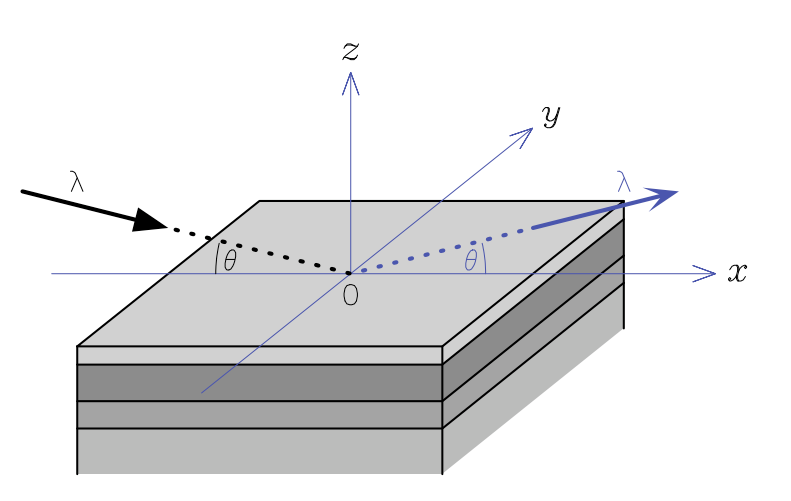
\includegraphics[width=0.85\textwidth]{theory/reflectgeo}
    \caption{A schematic showing the geometry of a typical specular reflectometry experiment from a layered sample. Reproduced, with permission of Oxford University Press\textsuperscript{\textcopyright}, from Reference~\cite{sivia_elementary_2011}.}
    \label{fig:refgeo}
\end{figure}
%
A reflectometry instrument operates by measuring the intensity of specular radiation at a series of different angles, $\theta$, or wavelengths, $\lambda$.
The reflected intensity is defined in terms of $q$ (by Equation~\ref{equ:theq}), and is defined as follows,
%
\begin{equation}
    R(q) = \frac{\text{specular reflected radiation intensity at }q}{\text{incident radiation intensity}}.
    \label{equ:refl}
\end{equation}
%
It is clear from Equation~\ref{equ:refl} that the value of the measured reflectometry cannot be greater than one, as this would mean that more particles of probing radiation were being reflected than were incident.

\subsubsection{Analysis}

There are two model-dependent analysis techniques that can be applied to the rationalisation of a reflectometry dataset.
The first is the kinematic approach, which can be obtained from Equation~\ref{equ:sca}, from the assumption that $q_x = 0$ and $q_y = 0$, as we are only measuring the specular scattering.
This approach models the reflectometry as a function of the scattering length density profile in the \emph{z}-dimension, $\rho(z)$,
%
\begin{equation}
    R(q) \approx \frac{16\pi^2}{q^4}\bigg|\int_{-\infty}^{+\infty}\frac{\text{d}\rho(z)}{\text{d}z}\exp{(-\mathbf{i}zq_z)}\text{d}z\bigg|^2,
    \label{equ:kine}
\end{equation}
%
where, $\sfrac{\text{d}\rho(z)}{\text{d}z}$ is the first derivative of the scattering length density profile.
However, this method has a significant problem, which can be demonstrated by applying Equation~\ref{equ:kine} to the scattering length density profile of a bare silicon substrate, which can be modelled as a Heaviside function (Figure~\ref{fig:kine}a),
%
\begin{equation}
    \rho(z) =
  \begin{cases}
    0, & \text{where}\ z < 0 \\
    \rho_{\text{Si}}, & \text{otherwise}
  \end{cases}
\end{equation}
%
where, $\rho_{\text{Si}}$ is the scattering length density of pure silicon (\SI{2.1e-6}{\angstrom^{-2}} for neutrons).
The derivative of a stepwise Heaviside function is a scaled $\delta$-function (Figure~\ref{fig:kine}b),
%
\begin{equation}
    \rho'(z) = \rho_{\text{Si}}\delta(z).
\end{equation}
%
Then, as in Equation~\ref{equ:kine}, the Fourier transform of this $\delta$-function is taken,
%
\begin{equation}
    \rho_{\text{Si}}\int_{-\infty}^{+\infty}\delta(z)\exp{(-\mathbf{i}zq_z)}\text{d}z = \rho_{\text{Si}}\exp(0) = \rho_{\text{Si}}.
    \label{equ:rhosi}
\end{equation}
%
This means that, using Equations~\ref{equ:rhosi} and \ref{equ:kine}, the reflectometry profile could be calculated from the following relationship,
%
\begin{equation}
    R(q)\approx \frac{16\pi^2\rho_{\text{Si}}^2}{q_z^4}.
\end{equation}
%
The curve from this relationship is shown in Figure~\ref{fig:kine}, where it is clear that the agreement with an experimental profile would be poor as $q \rightarrow 0$.
It can be seen that for low values of $q$ the calculated reflectometry is greater than 1, which violates the physical constraint imposed with Equation~\ref{equ:refl}.
This break down of the kinematic approach is due to the assumption present in this approach that the Born approximation (mentioned in Section~\ref{sec:multiscat}) will hold.
However, in the reflectometry scattering geometry, this is no longer true rendering the kinematic approach invalid.
%
\begin{figure}
    \centering
    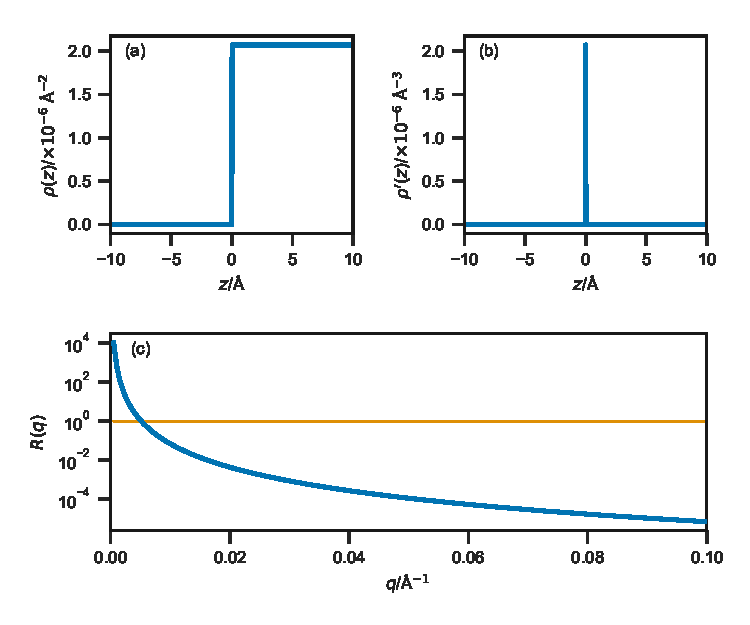
\includegraphics[width=0.85\textwidth]{theory/kine}
    \caption{A graphical representation of the kinematic approach; (a) the Heaviside function describing the scattering length density profile of a bare silicon substrate, (b) the $\delta$-function arising from the first derivative of the function in (a), and (c) the reflectometry profile resulting from Equation~\ref{equ:kine}, where the orange line at $R=1$ identifies the break down between experimental and theory in the kinematic approach. Adapted, with permission of Oxford University Press\textsuperscript{\textcopyright}, from Reference~\cite{sivia_elementary_2011}.}
    \label{fig:kine}
\end{figure}
%

This breakdown of the kinematic approach has led to the application of the Abel\`{e}s, or Parratt, model for the reflection of light at a given number of stratified interfaces (also known as dynamical theory) \cite{abeles_sur_1948,parratt_surface_1954}.
This method involves considering the system as a layered structure at the interfaces of which the probing radiation can either be reflected or refracted, by some refractive index, $n_i$.
Figure~\ref{fig:reflrefr} shows this process for a system of two layers, where the layer $0$ is the air or vacuum above the sample, it is clear to see how the two waves labelled $r$ could interfere constructively or destructively depending on the thickness of layer $1$, $d$.
This means that for a single interface, such as that between layers $0$ and $1$ in Figure~\ref{fig:reflrefr}, the reflectometry can be described by the Fresnel equation,
%
\begin{equation}
    R(q) = \bigg| \frac{n_0\sin{\theta_0} - n_1\sin{\theta_1}}{n_0\sin{\theta_0} + n_1\sin{\theta_1}} \bigg|^2.
\end{equation}
%
Additionally at the point of total reflection, where $\theta_0 = \theta_{\text{c}}$, the critical angle, there will be no transmitted wave so,
%
\begin{equation}
    n_1\sin{\theta_1} = 0,
\end{equation}
%
and therefore the reflected radiation will never be greater than 1, while the critical angle can be defined as,
%
\begin{equation}
    \cos^2{\theta_{\text{c}}} = \frac{n_1^2}{n_0^2}.
\end{equation}
%
This is the angle below which a reflectometry profile will be measured.
%
\begin{figure}
    \centering
    \includegraphics[width=0.85\textwidth]{theory/reflrefr}
    \caption{A schematic diagram showing the reflected ($r$) and transmitted ($t$) waves when an incident ($i$) wave enters an interface of thickness $d$, where the refractive indices of each layer are $n_0$, $n_1$, and $n_2$. Adapted from \cite{foglia_studies_2015}, with permission from Elsevier.}
    \label{fig:reflrefr}
\end{figure}
%

The above method can then be generalised to a structure of an arbitrary number of layers, as shown in Code Block~\ref{cb:refl}.
For each value of $q$ for which the reflectometry is to be calculated, the system is considered in terms of $n_{\text{max}}$ layers.
The incident radiation beam will be refracted by each of the layers, giving wavevectors values for each layer, $k_n$,
%
\begin{equation}
    k_n = \sqrt{k_0^2 + 4\pi (\rho_n - \rho_0)},
\end{equation}
%
where, $k_0=\sfrac{q}{2}$.
The Fresnel equation coefficient between layers $n$ and $n+1$, $r_{n,n+1}$ can then be found along with the phase factor, $\beta_n$, which is dependent on the thickness of the layer, $d_n$,
%
\begin{equation}
    r_{n,n+1} = \frac{k_n - k_{n+1}}{k_n + k_{n+1}},
    \label{equ:fres}
\end{equation}
%
%
\begin{equation}
    \beta_n = k_n d_n.
\end{equation}
%
The means that a matrix can be evaluated for each layer, $M_n$,
%
\begin{equation}
    M_n =
    \begin{bmatrix}
        \exp{\beta_n} & r_{n,n+1}\exp{-\beta_n} \\ r_{n,n+1}\exp{\beta_n} & \exp{-\beta_n}
    \end{bmatrix}
\end{equation}
%
The resultant matrix, $B_n$, is then found as a product of the matrix from each layer,
%
\begin{equation}
    B = \prod_{n=0}^{n_{\text{max}}} M_n,
\end{equation}
%
and from this the reflected intensity at the given value of $q$ can be found,
%
\begin{equation}
    R(q_z) = \frac{B_{1,2}}{B_{1,1}}.
\end{equation}
%
This algorithm models the layers as perfectly flat layers, which will not be strictly true in the case of soft matter systems such as a bilayer.
This resulted in the correction term being added to Equation~\ref{equ:fres} to account for the roughness of the layers.
This adapts Equation~\ref{equ:fres} to the form,
%
\begin{equation}
    r_{n,n+1} = \frac{k_n - k_{n+1}}{k_n + k_{n+1}}\exp{(-2k_nk_{n+1}\sigma^2_{n,n+1})},
\end{equation}
%
where, $\sigma_{n,n+1}$ is the interfacial roughness between layers $n$ and $n+1$.
This has the effect of Gaussian broadening the layers into each other, as a result. Code Block~\ref{cb:refl} is currently implemented in a variety of reflectometry modelling software packages, such as \texttt{refnx}, MOTOFIT, RasCAL, and Aurore \cite{nelson_refnx_2019,nelson_co-refinement_2006,hughes_rascal_nodate,gerelli_aurore_2016-1,gerelli_aurore_2016}.
Applying this method to the scattering length density profile shown in Figure~\ref{fig:kine} gives the reflectometry profile shown with the dashed green line in Figure~\ref{fig:dyna}.
%
\begin{figure}
    \centering
        \lstinputlisting[caption={An example Python code block for the Abel\`{e}s method for the calculation of reflectometry, adapted from Reference~\cite{nelson_refnx_2019}.},label={cb:refl}]{reports/code_blocks/reflectometry.py}
\end{figure}
%
%
\begin{figure}
    \centering
    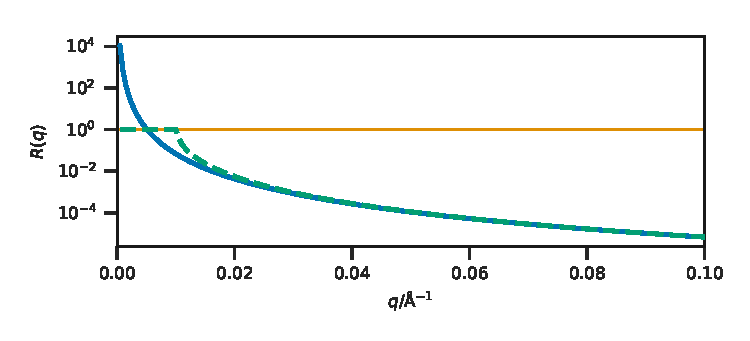
\includegraphics[width=0.85\textwidth]{theory/dyna}
    \caption{A comparison of the kinematic approach (blue solid line), and the dynamical approach (green dashed line), to determine the reflected intensity from the material with the scattering length density profile given in Figure~\ref{fig:kine}(a). It is clear that at low $q$, there is a noticable deviation between the two.}
    \label{fig:dyna}
\end{figure}
%


\subsection{Small angle scattering}
\label{sec:sasanal}

Equation~\ref{equ:sldsca} identified that the scattering differential cross-section for some object was related to the scattering length density by a Fourier transform, which is shown graphically in Figure~\ref{fig:scales}.
This figure shows that there is a reciprocal relationship between the size of the object and the scattered intensity, decaying significantly up to values of $2\pi/d_x$, where $d_x$ is the size of the object.
This means that in order to probe the large-scale structural features that are of interest in the study of soft materials, it is necessary to consider small values of $q$.
When considering the nature of $q$ in Equation~\ref{equ:theq}, it is clear that such experiments would benefit from small values of $\theta$ and large values of $\lambda$.
Hence, the application of small angle scattering (SAS).
%
\begin{figure}
    \centering
    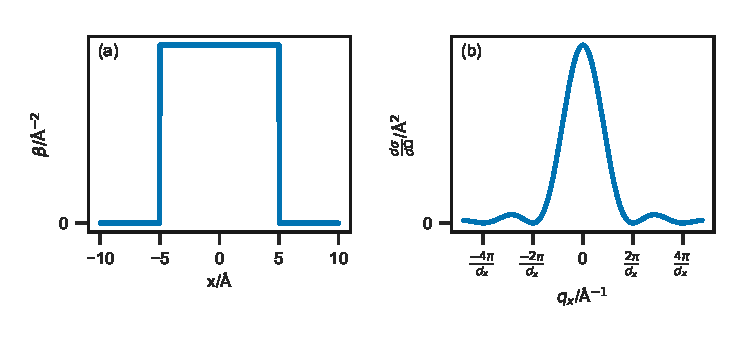
\includegraphics[width=0.85\textwidth]{theory/scales}
    \caption{The effect of a Fourier transform (a) the scattering length density profile for some object with a width of \SI{10}{\angstrom}, (b) the Fourier transform of this object showing the minima in the differential cross section at values of $\sfrac{2n\pi}{10}$, where $n$ is some integer.}
    \label{fig:scales}
\end{figure}
%

A SAS experiment generally involves some sample being placed in the path of the probing radiation; the scattering pattern that results from this transmission is measured at some distance, as is shown in Figure~\ref{fig:sasgeo} for the D22 SANS instrument of the ILL.
SAS instruments are usually very large, due to the large post sample flight path that is necessary to reach the small angles being measured; a longer flight path allows more space for angular divergence.
Transmission SAS can provide information about the size, shape and orientation of the sample's components \cite{willis_experimental_2009}.
The range in $q$ that is typically covered by a SAS instrument is usually around \SIrange{2e-3}{0.5}{\per\angstrom}, which corresponds to \SIrange{10}{3000}{\angstrom} in real-space. The neutron or X-ray detector of a SAS instrument is often two-dimensional, meaning that for an isotropic scattering profile, the detector image is radially averaged to give an $I(q)$ scattering profile.
It is possible to increase the $q$-range of a SAS instrument through the introduction of wide-$q$ detector banks close to the sample or small-$q$ detector banks further away.
This allows the SANS2D instrument, at the ISIS Neutron and Muon Source, to have a total range from \SIrange{2e-3}{2}{\per\angstrom} \cite{noauthor_isis_nodate}.
Furthermore, the SANS2D instrument may leverage the time-of-flight method discussed in Section \ref{sec:neutrons} to allow for a much shorter post sample flight path than is present at D22.
%
\begin{figure}
    \centering
    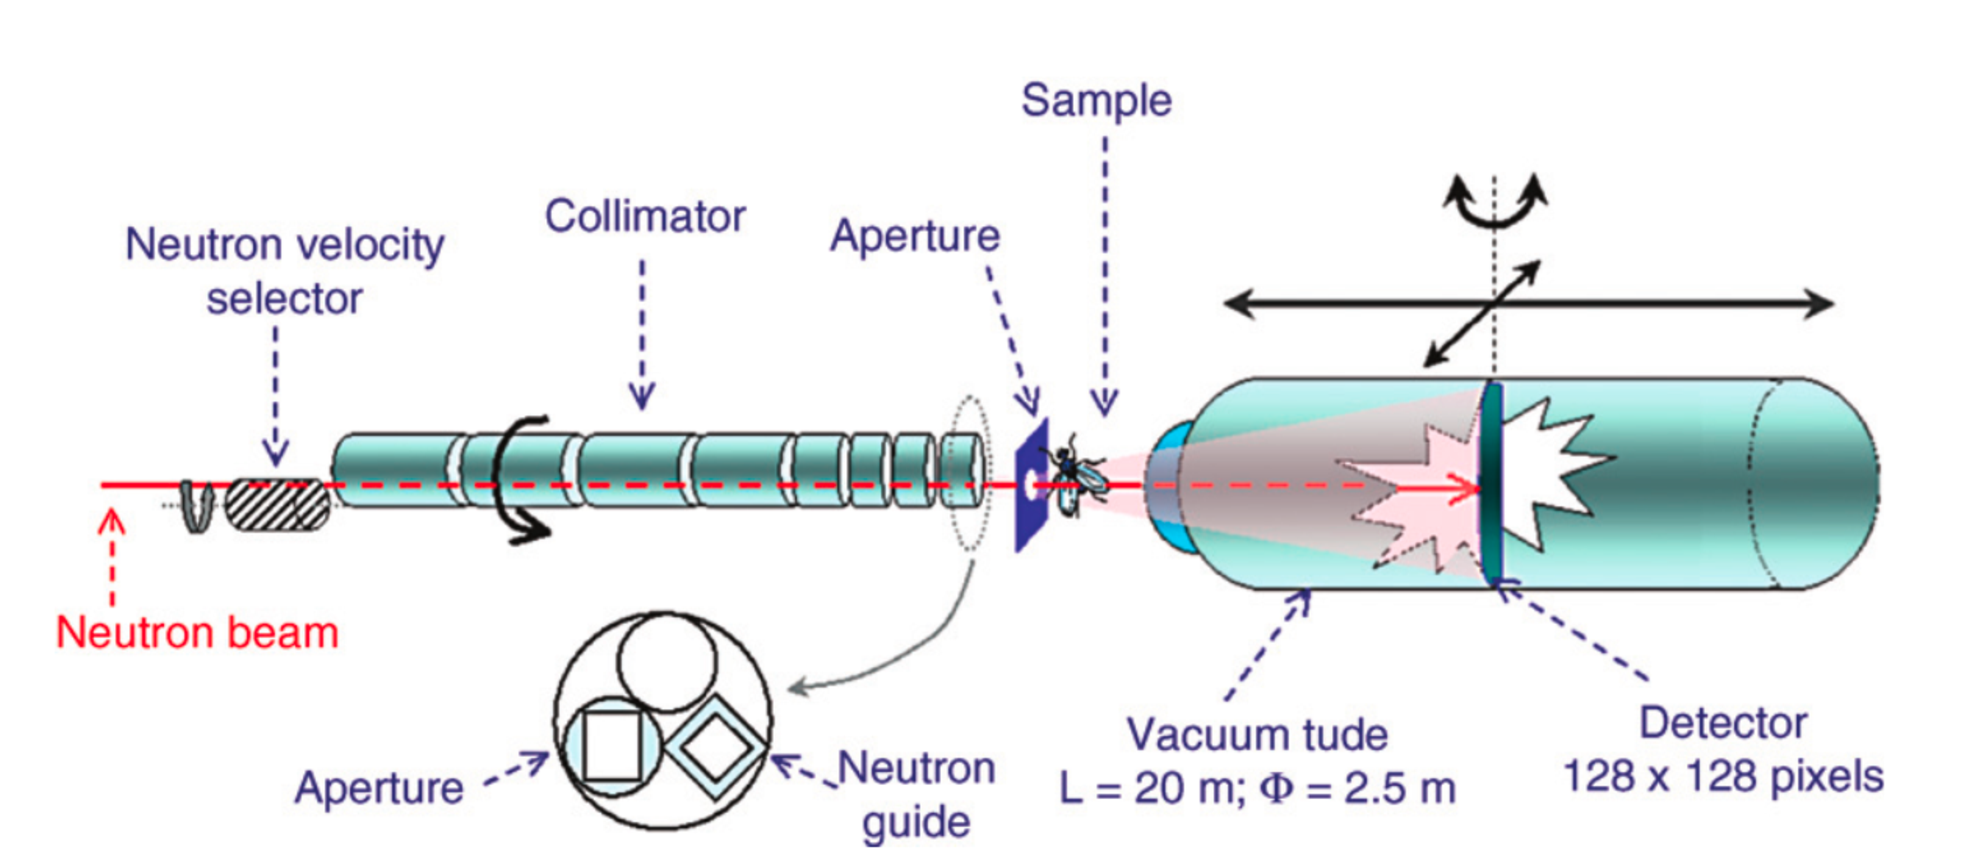
\includegraphics[width=0.85\textwidth]{theory/d22}
    \caption{A schematic of the D22 instrument of the ILL, from Reference~\cite{grillo_small-angle_2008}. Reprinted/adapted by permission from Springer Nature Customer Service Centre GmbH: Springer Nature Small-Angle Neutron Scattering and Applications in Soft Condensed Matter by I. Grillo\textsuperscript{\textcopyright} (2008).}
    \label{fig:sasgeo}
\end{figure}
%

\subsubsection{Analysis}

A radially averaged SAS pattern can be considered as consisting of two sections that arise from the form and structure factors for the scattering species.
The form factor gives information about the average shape of the scattering particle, while the structure factor is a measure of the interaction present between the objects.
It is often possible to control the presence of the structure factor by changing the concentration of the sample, eventually, the concentration will be so low that all interparticle interaction is screened by the solvent \cite{edler_combining_2015}.
This method is frequency applied in BioSAXS applications, where the interactions between the protein molecules are of less interest than the overall structure of the complex.
However, with micelles, it is not always possible to remove the structure factor, as the critical micelle concentration may be higher than the minimum concentration at which the structure factor is present.
It is possible to deconvolute the structure and form factors for a micellar solution by studying different concentrations, assuming that the form of the micelle is concentration independent, over the measured concentration range.

The rigorous, model-independent method for the analysis of SAS involves taking the inverse Fourier transform of the scattering profile, to give an auto-correlation function of the average particle in the system, which following a deconvolution procedure will resolve the radially averaged scattering length density profile.
However, this is often cumbersome and has a low information density, when compared to model-dependent techniques.
Additionally, if the experimental data lacks information at wide enough $q$ to cover all features of the sample, artefacts may be present in the inverse Fourier transform of the scattering.

There are two common and straight-forward analysis procedures that can be used to give an understanding of the scattering species structure.
The first is the Guinier approximation, which is used in the determination of the radius of gyration, $R_g$, of the scattering species, at ``infinite dilution''.
This scattering law is only valid at very small values of $q$, where $q < R_g^{-1}$ \cite{sivia_elementary_2011},
%
\begin{equation}
    \ln[I(q)] = \ln[I(0)] - \Bigg(\frac{R_g^2}{3}\Bigg)q^2.
\end{equation}
%
This relationship allows the radius of gyration to be found by plotting the scattering profile transformed into $\ln[I(q)]$ vs. $q^2$, and evaluating the gradient at low $q$.
The Guinier plot for the scattering from a sphere with a radius of \SI{20}{\angstrom} is shown in Figure~\ref{fig:rg}, where the radius of gyration correlates with the radius of the sphere, $R$, as follows,
%
\begin{equation}
    R_g = \sqrt{\frac{3}{5}}R.
\end{equation}
%
The Guinier analysis is very common in the study of proteins by SAS, as it allows for the determination of the protein size in the native, solution phase \cite{skou_synchrotron-based_2014}.
Another common analysis of SAS data comes in the form of Porod's law, which states that for large values of $q$, the scattering intensity becomes proportional to $Sq^{-4}$, where $S$ is the surface area of the sample.
This means that by plotting $I(q)q^4$ vs. $q$ and extrapolating to $q \rightarrow \infty$, it is possible to determine the external surface area of the system \cite{willis_experimental_2009}.
Using the surface area, it is then possible to qualitatively determine the `roughness' of the system based on the relation of the surface area to the particle size.
%
\begin{figure}
    \centering
    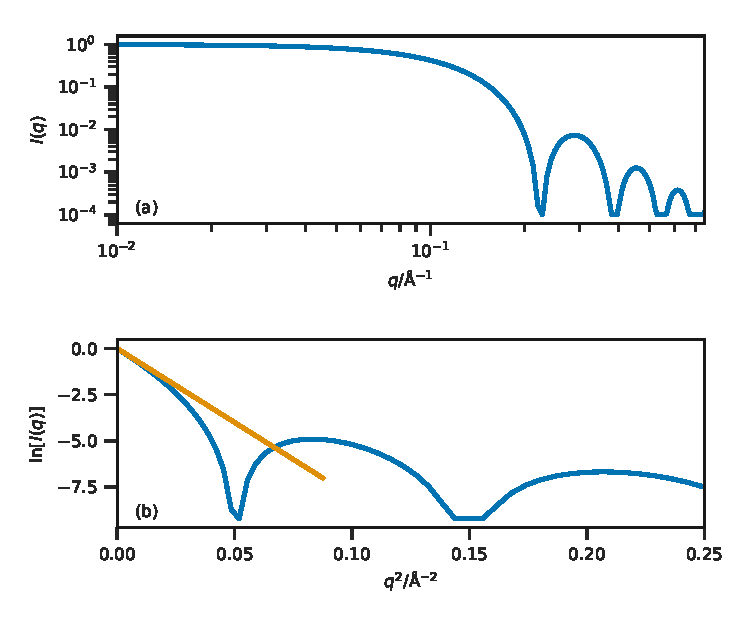
\includegraphics[width=0.85\textwidth]{theory/rg}
    \caption{The Guinier plot, (a) the ideal scattering profile from a sphere of radius \SI{20}{\angstrom}, (b) the associated Guinier plot, with a straight line (orange) at low-$q$ showing the radius of gyration to be \SI{\sim15.5}{\angstrom}.}
    \label{fig:rg}
\end{figure}
%

In the calculation of a SAS pattern, both the structure and form factors will contribute.
Therefore, when we model the pattern, the differential cross-section has the following form, when the system is centrosymmetric.
%
\begin{equation}
    \frac{\text{d}\sigma(q)}{\text{d}\Omega} = N_\rho\Delta\rho^2V_p^2 P(q)S(q),
\end{equation}
%
where $N_\rho$ is the number density of the particles, $\Delta\rho$ is the difference in scattering length density between the particles and the solvent, $V_p$ is the particle volume, $P(q)$ is the particle form factor, and $S(q)$ is the structure factor \cite{pedersen_monte_2002}.
Therefore, it is necessary to understand how the function of the form factor and structure factor come to be.

The most common method for the modelling of the form-factor is by using very coarse shapes; such as spheres, cylinders, or ellipses.
This involves the evaluation of analytical or quasi-analytical solutions for the scattering, which have been derived for many common shapes.
The solution for a sphere was solved in the early 19th century by Lord Rayleigh \cite{pedersen_monte_2002}.
%
\begin{equation}
    P(q) = \Bigg\{\frac{3\big\{\sin(qR) - qR\cos(qR)\big\}}{(qR)^3}\Bigg\}^2,
    \label{equ:sphere}
\end{equation}
%
where $R$ is the radius of the sphere. A comparison between a possible experimental scattering pattern and the scattering generated from Equation~\ref{equ:sphere} is shown in Figure~\ref{fig:sphere}. Analytical form factors exist for a wide variety of shapes; these can be found in software such as SASView and SASFit \cite{noauthor_sasview_nodate, noauthor_sasfit_nodate}.
%
\begin{figure}
    \centering
    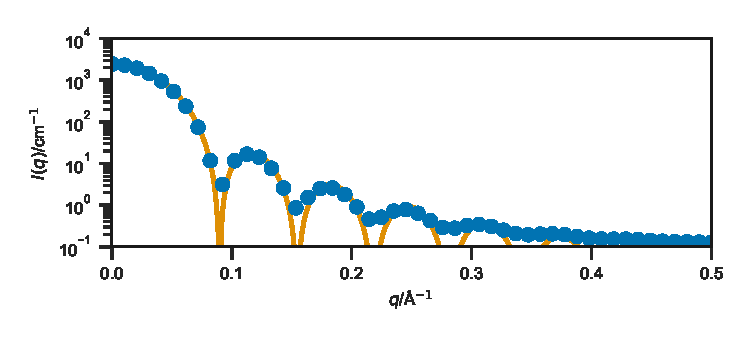
\includegraphics[width=0.85\textwidth]{theory/sphere}
    \caption{The SANS profile of a micelle of \ce{C_{16}TAB} with radius $\SI{50(3)}{\angstrom}$ (circles, generated using SASView \cite{noauthor_sasview_nodate}, with instrumental smearing) compared with a curve of Equation~\ref{equ:sphere}, where $R = \SI{50}{\angstrom}$ (solid line).}
    \label{fig:sphere}
\end{figure}
%

The structure factor accounts for the scattering interference that arises from the interaction of different particles.
This is modelled using expressions which depend on the nature of the scattering particles; hard-sphere, sticky hard-spheres, screened Coulomb, etc.
Structure factor expressions are generated as solutions to the Ornstein-Zernike Equation~\cite{klein_interacting_2002}.
The most relevant structure factor in terms of micelle modelling is probably the Hayter-Penfold Mean Spherical Approximation \cite{hayter_analytic_1981}, this is where the micelles are modelled as like-charged, soft spheres and is valid for dilute solutions.
Again, a whole range of these structure factor functions are built into the SASView package \cite{noauthor_sasview_nodate}.

In order to evaluate the scattering profile from an atomic, or coarse-grained system, it is possible to use the Debye equation \cite{debye_zerstreuung_1915}.
This is an analysis relation for the determination of the scattering profile based on the atomic positions, $\mathbf{r}_i$,
%
\begin{equation}
    I(q) = \sum_{i}^{N}\sum_{j}^{N} b_ib_j\frac{\sin{(q|\mathbf{r}_i-\mathbf{r}_j|)}}{q|\mathbf{r}_i-\mathbf{r}_j|},
\end{equation}
%
where, $N$ is the number of particles, $q$ is the scattering vector, and $b_i$ and $b_j$ are the scattering lengths of particles $i$ and $j$ respectively, for a coarse-grained particle this can be obtained from summing the scattering lengths of the constituent atoms.
The Debye equation is powerful, however, it is not intrinsically parallelisable and as a result scales as $\mathcal{O}(N^2)$.
In order to improve the efficiency of the calculation of the scattering profile, a variety of methods have been developed that offer a sufficiently accurate approximation \cite{svergun_solution_1994,watson_rapid_2013}.
The Golden Vector method, developed by Watson and Curtis \cite{watson_rapid_2013} scales as $\mathcal{O}(Nn)$, where $n$ is the number of scattering vectors used in the calculation.
In this method, the scattering amplitude is calculated numerically for a single $\mathbf{q}$-vector,
%
\begin{equation}
    I(\mathbf{q}) = \Bigg[\sum_{i}^{N}b_i\cos{(\mathbf{q}\cdot\mathbf{r}_i)}\Bigg]^2 + \Bigg[\sum_{i}^{N}b_i\sin{(\mathbf{q}\cdot\mathbf{r}_i)}\Bigg]^2.
\end{equation}
%
This is carried out for $n$ scattering vectors that are selected in an orientationally averaged fashion from a quasi-uniform lattice on a sphere.
This was first developed such that $n$ is a number from the Fibonacci sequence \cite{svergun_solution_1994}, however for the Golden Vector method, $n$ may be any positive integer.
This leads to the scattering vectors being calculated as,
%
\begin{equation}
    \begin{aligned}
        q_x^{(k)} & = q\cos\Bigg[\sin^{-1}\bigg(\frac{2k}{n}\bigg)\Bigg]\cos\bigg(\frac{2\pi k}{\Phi}\bigg), \\
        q_y^{(k)} & = q\cos\Bigg[\sin^{-1}\bigg(\frac{2k}{n}\bigg)\Bigg]\sin\bigg(\frac{2\pi k}{\Phi}\bigg), \\
        q_z^{(k)} & = \frac{2 k q}{n},
    \end{aligned}
\end{equation}
%
where, $k$ runs from $-(n-1)/2,\ldots,0,\ldots,(n-1)/2$ and $\Phi$ is the golden ratio,
%
\begin{equation}
    \Phi = \frac{1+\sqrt{5}}{2}.
\end{equation}
%
The approximate orientationally averaged scattering is then found as an average of the scattering from each of ther individual $q$-vectors,
%
\begin{equation}
    I(q) = \frac{1}{n}\Bigg\{\sum_{k=(1-n)/2}^{(n-1)/2} I[\mathbf{q}^{(k)}]\Bigg\}.
\end{equation}
%
The accuracy of this calculation increases with $n$, however agreement, comparible to the Debye equation, between experiment and simulation has been shown for $n < 100$ even for highly anisotropic systems \cite{watson_rapid_2013}.


%\subsection{Grazing incidence small angle scattering}

%While reflectometry is the study of specular reflections from a layer structure, grazing incidence small angle scattering (GISAS) is the study of the off-specular reflections, those where the scattering vector has $x$- and $y$-components in addition to the $z$-component.
%This off-specular scattering is that which arises from the heterogeneity present at the interface.
%This means that GISAS is ideal for the study of material with nanostructure in the plane of the interface, such as organic semiconducting materials or polymer-grafted nanoparticles at an interface \cite{muller-buschbaum_local_2005,zhang_ion-specific_2017}.
%The geometry of a GISAS experiment on a thin film material is shown in Figure~\ref{fig:gisas}, which also shows a typical GISAS pattern.
%
%\begin{figure}
%    \centering
%    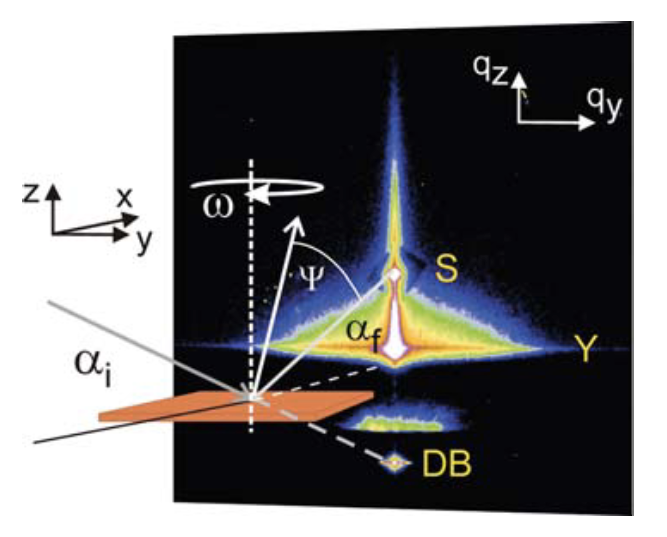
\includegraphics[width=0.85\textwidth]{theory/gisas}
%    \caption{A schematic of the geometry of a GISAS experiment, where $\alpha_i$ is the incident angle, $\alpha_f$ is the exit angle, and $\phi$ is the out-of-plane angle, from Reference~\cite{muller-buschbaum_basic_2009}. Reprinted/adapted by permission from Springer Nature Customer Service Centre GmbH: Springer Nature A Basic Introduction to Grazing Incidence Small-Angle X-Ray Scattering by P. M\"{u}ller-Buschbaum\textsuperscript{\textcopyright} (2009).}
%    \label{fig:gisas}
%\end{figure}
%

%In terms of GISAS instrumentation, it can be considered as an amalgamation of a reflectometry instrument and a small angle scattering instrument.
%The sample environment is that from a reflectometry instrument, while the two-dimensional detector required is that commonly associated with small angle scattering.
%Commonly, GISAS is found as an additional capability of another instrument, such as the grazing incidence small angle neutron scattering (GISANS) capability of D22 at the ILL or the GISAS setup at I07 of the Diamond Light Source \cite{muller-buschbaum_grazing_2004,nicklin_diamond_2016}.
%However, as GISAS has grown in popularity as a technique, GISAS focused instruments have been installed, such as MiNaXS at DESY in Hamburg and Beamline 7.3.3 at the ALS in San Francisco \cite{buffet_p03_2012,hexemer_saxs/waxs/gisaxs_2010}.

%\subsubsection{Analysis}

%The analysis process for a GISAS pattern is substantially more complex than for either the SAS or reflectometry counterparts.
%This is due to the fact that for SAS, the Born approximation is conserved, and only a single scattering event is considered.
%While for reflectometry, there is a well defined theoretical background that enables the analysis where the Born approximation is not valid.
%This is not the case for GISAS since for off-specular reflectometry to occur, the probing radiation will undergo both scattering and reflectometry events simultaneously.
%In order to account for this, generally, the distorted wave Born approximation (DWBA) is invoked.
%This is an extension of the Born approximation, wherein there are four possible ways in which the probing radiation may interact with the material, these are shown in Figure~\ref{fig:dwba}.
%
%\begin{figure}
%    \centering
%    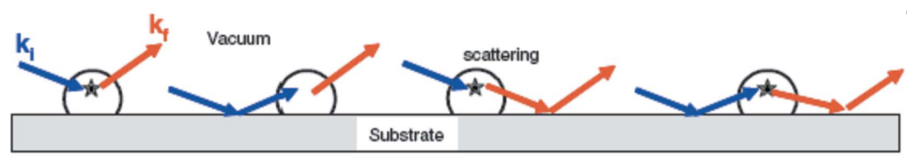
\includegraphics[width=0.85\textwidth]{theory/dwba}
%    \caption{The four possible way in which some probing radiation may interact with a sample within the DWBA; scattering, reflection-then-scattering, scattering-then-reflection, and reflection-then-scattering-then-reflection, from Reference~\cite{hexemer_advanced_2015}.}
%    \label{fig:dwba}
%\end{figure}
%

%One of the most common methods for the analysis of a GISAS pattern is Bragg peak analysis.
%This is where Bragg peaks of crystallinity in the GISAS pattern are selected and analysed in terms of Bragg's and Snell's laws to account for the effects of the surface and substrate, this allows the dependence of $q_z$ to be determined \cite{lee_electron_2007, busch_grazing-incidence_2006}.
%While useful, this analysis approach is limited to systems with high crystallinity, such as stacked lamellae \cite{busch_inner_2007}.
%This method cannot be easily applied to understand less organised arrangements in soft matter systems, as these give rise to broad, smeared peaks with no clear centre.

%Another simplified method for the analysis of a GISAS pattern involves the effective surface approximation.
%This is where, from the two-dimensional GISAS pattern, selected cuts are taken and analysed only as a function of $q_y$.
%This can be used to probe depth-dependent properties, as taking such a cut effectively considered the lateral structure at a given depth, rather than both the lateral structure and that normal to the interface.
%For incident angles $\alpha_i \gg \alpha_c$ and at constant $q_z$, the scattering intensity in the DWBA simplifies and the differential cross section is given by \cite{naudon_grazing-incidence_2000},
%
%\begin{equation}
%    \frac{\text{d}\sigma}{\text{d}\Omega} = \frac{A\pi^2}{\lambda^4}\big[(1 - n^2)T_iT_f\big]^2F(\mathbf{q}),
%\end{equation}
%
%where $A$ is the iluminated surface area, $T_{i,f}$ are the Fresnel transmission factors for incidence and reflectance, and $F(\mathbf{q})$ is the diffuse-scattering factor, which is dependent on the form and structure factors of the lateral structure.

%Currently, there exists a handful of software packages that are designed to aid in the structural analysis by GISAS.
%These include, but are not limited to, IsGISAXS, BornAgain, and HipGISAXS \cite{lazzari_isgisaxs_2002,burle_bornagain_nodate,chourou_hipgisaxs_2013}.
%These software packages generally implement analytical solutions to the DWBA by considering different form and structure factors for some system.
%In order to have some understanding of the structure that should be fitted to the experimental data, it is often necessary to perform electron microscopy measurements to educate the analysis process.


\subsection{Contrast variation}
\label{convar}

The scattering profile generated by the interaction of the chosen system with radiation depends on three factors:
%
\begin{itemize}
    \item the spatial arrangement of the atoms in the system,
    \item the instrument being used to measure the pattern; instrumental resolution function, and
    \item the interaction between the radiation and the matter under investigation.
\end{itemize}
%
This final factor is perhaps better known as the `scattering contrast', this is an extremely important factor in the study of soft matter, particularly when the probing radiation is the neutron.
The scattering contrast makes it possible to select individual components of the system and investigate their structural properties \cite{schurtenberger_contrast_2002}.
The differential cross-section, $\sfrac{\text{d}\sigma}{\text{d}\Omega}$ of a point scatterer, as shown in Equation~\ref{equ:sca}, varies only with respect to the scattering length of the species, $b$,
%
\begin{equation}
    \frac{\text{d}\sigma}{\text{d}\Omega} \propto b^2.
\end{equation}
%
However, as discussed in Section~\ref{sec:sld}, it is often easier to use the scattering length density, $\rho$.

When an X-ray interacts with an atom, it is scattered by the interaction with the electrons, this is due to the X-ray being a form of electromagnetic radiation.
Furthermore, it means that the scattering length of an atom by an X-ray is directly proportional to the number of electrons in the atom, so it is therefore difficult to discern between the scattering from a carbon atom (6 electrons) and a nitrogen atom (7 electrons), furthermore the scattering from hydrogen atoms is practically non-existent, in comparison.

The scattering length from neutrons varies nonsystematically with respect to the atomic number of a species, this is shown in Figure~\ref{fig:scatlen}.
Furthermore to the apparently random variation with changes in atomic number, there is also significant variation with mass number, e.g. between isotopes of the same atom.
There is also dependence due to the magnetic state of the atom, however, this is normally unimportant for soft matter.
The scattering lengths differ with the nuclear spin energy level, this leads to an average scattering length, $\langle b \rangle$, for isotopes where the nuclear spin is non-zero ($S\neq 0$).
There are two forms of scattering, coherent and incoherent, for which the scattering cross-sections, $\sigma$, are determined by,
%
\begin{equation}
    \begin{aligned}
        \sigma_{\text{coh}} & = 4\pi\langle b \rangle ^2 \\
        \sigma_{\text{incoh}} & = 4\pi(\langle b ^ 2 \rangle - \langle b \rangle ^2) \\
    \end{aligned}
\end{equation}
%
The coherent scattering is the scattering from nuclei that all have the same value of $b$, and leads to the important scattering pattern.
Whereas, the incoherent scattering is caused by the `disorder' between the isotopes, and is the cause of the background present in the measurement.
Examples of these scattering cross-sections for nuclei relevant to soft matter are shown in Table \ref{tab:crosssec}.
It can be seen that the incoherent scattering from the \ce{^1H} nuclei is more than forty times higher than the coherent scattering.
This leads to a large, intrusive background present in the scattering pattern of hydrogenous samples.
%
\begin{figure}
    \centering
    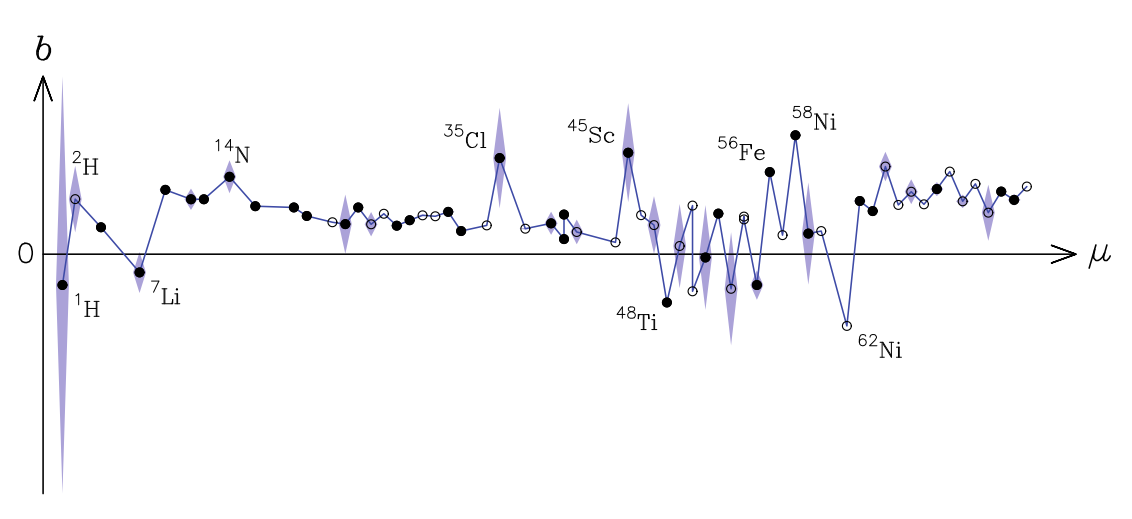
\includegraphics[width=0.85\textwidth]{theory/scatlen}
    \caption{The variation of the average neutron scattering length, $\langle b \rangle$ (circles), with atomic mass, $\mu$. The standard deviation, $\Delta b$, is indicated with the shaded regions. Reproduced, with permission of Oxford University Press\textsuperscript{\textcopyright}, from Reference~\cite{sivia_elementary_2011}.}
    \label{fig:scatlen}
\end{figure}
%
\begin{table}
    \centering
    \small
    \caption{Examples of coherent and incoherent scattering cross-sections, from Reference~\cite{schurtenberger_contrast_2002}.}
    \label{tab:crosssec}
    \begin{tabular}{r | c c c}
        \toprule
        Isotope & $S$ & $\sigma_{\text{coh}}$/\SI{e-28}{\meter\square} & $\sigma_{\text{incoh}}$/\SI{e-28}{\meter\square} \\
        \midrule
        \ce{^1H} & $\sfrac{1}{2}$ & 1.8 & 79.7 \\
        \ce{^2H} & 1 & 5.6 & 2.0 \\
        \ce{^{12}C} & 0 & 5.6 & -- \\
        \ce{^{14}N} & 1 & 11.6 & 0.3 \\
        \ce{^{16}O} & 0 & 4.2 & -- \\
        \bottomrule
    \end{tabular}
\end{table}
%

The difference between the scattering of \ce{^1H} and \ce{^2H}, evident in Table \ref{tab:crosssec}, can lead to a very useful technique in soft matter scattering, known as contrast variation.
The idea of contrast variation is based on the substitution of one isotope of an atom for another, while not introducing significant change to the properties of the material.
Traditionally the benefit of this came in terms of contrast matching out a part of the system to reduce the dimensionality of the problem for analysis.
For example, by matching the solvent scattering length density to that of the tails of the surfactants at the centre of a micelle there would only be scattered from the heads, and conversely, there would only be scattered from the tails if the solvent had the same scattering length density as the head groups.
This means that the problem becomes more straightforward as there are fewer variable parameters when fitting the data. This idea is represented graphically in Figure~\ref{fig:convar}.
%
\begin{figure}
    \centering
    \includegraphics[width=0.85\textwidth]{theory/convar}
    \caption{The effect of varying the scattering length density of the solvent in a micelle system, (a) the system in a pure solvent, (b) the solvent is contrast matched to the surfactant tails, and (c) the solvent is contrast matched to the surfactant heads.}
    \label{fig:convar}
\end{figure}
%
The technique of contrast variation may also be used in terms of data analysis.
By increasing the number of data sets corresponding to a single model at different contrasts, the solution for the true structure of the model from the scattering data becomes more robust.
This is due to the fact that each different contrast can be considered as an independent measurement of the same system, and hence each set of scattering data can be used within the data analysis procedure to obtain the best global agreement to the experiment.
This co-refinement of multiple experiments can, under the right conditions, be used to simultaneously consider both neutron and X-ray datasets \cite{nelson_co-refinement_2006}.

There is also the possibility of using contrast variation when the probing radiation is the X-ray, through the use of anomalous scattering.
This is where different wavelengths of radiation give different scattering when the wavelengths are on opposite sides of an X-ray absorption edge.
This is not frequently used for soft matter species, as the X-ray absorption edges for elements common in soft matter (H, C, N, O, etc.) are at very low X-ray energies so generally outside of the accessible range of a standard SAXS instrument \cite{schurtenberger_contrast_2002}.
